\section{Introduction}
\begin{frame}{Introduction}
\begin{columns}
\begin{column}{0.5\textwidth}
Motivation
\begin{itemize}
    \item \textit{S. cerevisiae}
    \item Systems biology approach
% Understanding the complexities of life has shown to be challenging. Gene regulation and protein interaction is at the core of shaping the function of any living cell. The interaction networks of proteins and metabolites inside a single cell are complex and ever changing, and it is not always trivial to understand how changes to one or more parts of the network will affect the overall. 
\end{itemize}

The problem
\begin{itemize}
    \item ORFs: 5178 verified, 737 uncharacterized, 689 dubious~\cite{YeastOverview}
    \item TFs: $\sim209$~\cite{Hughes2013}, PKs: $\sim129$~\cite{Rubenstein2007}, PPs: $\sim30$~\cite{Breitkreutz2010}
% Numbers of genes, transcription factors, and protein kinases are still not exactly defined. \textit{S. cerevisiae} currently has 5178 verified open reading frames~(ORFs), 737 uncharacterized ones, and 689 dubious ones~\cite{YeastOverview}.
% Estimated numbers of transcription factors vary from 141 to 251. If we define a transcription factor protein as a protein that binds DNA with sequence-specificity and regulates transcription nearby, then one estimate puts the number of known and putative TFs at 209~\cite{Hughes2013}. Putative refers to proteins that encode DNA-binding domains, and where their regulatory role is not unproven. A count of 127~protein kinases have been studied by Rubenstein~et~al.~\cite{Rubenstein2007}, while 129~protein kinases and 30~phosphatases were characterized by Breitkreutz~et~al.~\cite{Breitkreutz2010}.

    \item Graph learning combining different data types
% to model a cell as a graph to predict how it behaves under different conditions, we first need to infer the graph.
% Studying the abundance of interaction in a cell requires high throughput measurements which still come with the cost of high noise levels. High throughput RNA measurements has become cheaper at an increasing rate and can help in understanding direct protein interactions, as a supplement to directly assaying protein-protein and protein-DNA interaction.
% Since some data types such as RNA measurements are not direct assays of protein-protein and protein-DNA interactions, researchers in the field of systems biology study mathematical models, graph theory, and machine learning to develop ways to take advantage of all the different types of biological data available.
% Inferring graph structure has been examined extensively, each method with different assumptions and limitations. Here, we will try to examine graph structure inference specifically for the case of regulatory networks, and by using data from knockout studies.
\end{itemize}
\end{column}

\begin{column}{0.5\textwidth}
\begin{figure}[ht]
  \centering
  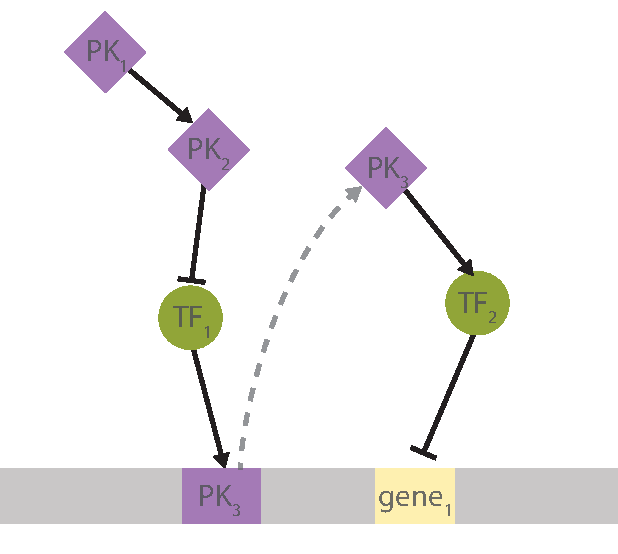
\includegraphics[width=0.7\textwidth]{introduction/fig/problem.pdf}
  \caption{\textbf{Gene regulation.}
  $\pk_1$ regulating $\gene_1$ indirectly through a cascade.}
  \label{fig:problem}
\end{figure}
\end{column}
\end{columns}
\end{frame}

